\chapter{Descrizione del progetto}
\label{cap:descrizione-progetto}

Il focus del progetto è l’analisi delle parole chiave, ma non in un’ottica di marketing: non vengono infatti considerati parametri come efficacia, \textit{ranking}, \gls{keyword-difficulty}, né funzionalità avanzate come anteprime \gls{serp} o suggerimenti di parole chiave. Questi aspetti dell’analisi \gls{seo}, sia \gls{on-page} che \gls{off-page}, sono già ampiamente supportati da numerose estensioni, gratuite e a pagamento, e pertanto non rappresentano una sfida particolarmente stimolante per uno progetto di stage. Inoltre, l’analisi del posizionamento di un sito per una determinata parola chiave richiede che il sito sia stato effettivamente pubblicato; di conseguenza, questa funzionalità non si adatta allo scopo dell’estensione, che è rivolta principalmente agli sviluppatori e deve quindi funzionare anche in ambiente \gls{localhost}. Al contrario, funzionalità come l’analisi della distribuzione delle parole chiave e la loro evidenziazione visiva all’interno della pagina, rientrano pienamente nell’analisi \gls{on-page} e rispondono a una necessità reale di molti sviluppatori. Tali funzionalità sono implementate separatamente in estensioni web come \textit{MozBar} o \textit{SEOquake}, ma difficilmente vengono integrate all’interno di un unico strumento. Tra i più noti, probabilmente solo il plugin \textit{Yoast SEO} per \gls{wordpress} consente sia l’analisi che l’evidenziazione delle parole chiave; tuttavia, come suggerisce il nome, si tratta di uno strumento pensato esclusivamente per sviluppatori che utilizzano un \gls{cms}. Pertanto, l’obiettivo del progetto è combinare queste due funzionalità in un’estensione web direttamente accessibile sin dalle prime fasi di sviluppo.

\section{Analisi preventiva dei rischi}
\label{sec:rischi}

Durante le discussioni iniziali con la Proponente, sono emersi alcuni rischi che, se non prevenuti o mitigati correttamente, potevano compromettere l’esito del progetto e il rispetto delle scadenze. Di seguito sono illustrati i rischi identificati e le relative strategie di prevenzione e/o mitigazione.

\begin{risk}{Risultato non conforme alle aspettative}
  \riskdescription{Trattandosi di uno stage interno, la Proponente ha evidenziato il rischio che, in caso di mancanza di feedback costanti, la soluzione sviluppata, in termini tecnici o di interfaccia grafica, non soddisfi le attese}
  \riskprevention{È prevista la creazione di una cartella documentale condivisa su Google Drive, aggiornata costantemente, che la Proponente può monitorare e commentare durante lo svolgimento del progetto.\\ Il \gls{repository} \gls{github} deve essere accessibile pubblicamente, al fine di consentire l’esecuzione di test manuali in parallelo a quelli automatici.\\ Sono previsti aggiornamenti periodici, in presenza o da remoto, con una frequenza di almeno una o due volte a settimana. In caso di aggiornamento a distanza, la comunicazione via e-mail deve risultare sufficientemente esaustiva}
  \label{risk:risultato-non-conforme} 
\end{risk}

\begin{risk}{Performance dell’estensione}
  \riskdescription{Per migliorare l'affidabilità dell’analisi delle parole chiave, potrebbe essere necessario sviluppare algoritmi più complessi dal punto di vista computazionale. Una volta integrate le nuove funzionalità nel progetto preesistente, le performance potrebbero non risultare ottimali, poiché quest’ultimo esegue già operazioni onerose, come l’analisi delle immagini}
  \riskprevention{Prima di sviluppare algoritmi che privilegino l’affidabilità a scapito delle prestazioni, lo stagista è tenuto a inviare alla Proponente una comunicazione via e-mail contenente un confronto, in termini di pro e contro, tra la soluzione attuale e quella proposta. Tale comunicazione deve includere esempi pratici basati su analisi e \textit{benchmarking}, lasciando alla Proponente la decisione finale in funzione degli obiettivi del progetto}
  \riskmitigation{Nel caso in cui il calo delle performance si verifichi comunque, lo stagista e la Proponente devono organizzare un incontro per individuare una soluzione che garantisca il giusto compromesso tra affidabilità e prestazioni}
  \label{risk:prestazioni} 
\end{risk}

\begin{risk}{Sottostima del tempo necessario}
  \riskdescription{Il preventivo “a finire” potrebbe comportare uno sforamento della scadenza prevista}
  \riskmitigation{Revisione e riformulazione dei \gls{requisiti} obbligatori minimi, al fine di garantire il raggiungimento degli obiettivi previsti ed evitare sforamenti eccessivi}
  \label{risk:scadenze} 
\end{risk}

\begin{risk}{Integrazione in un progetto preesistente}
  \riskdescription{L’integrazione dello strumento di analisi delle parole chiave in un progetto preesistente potrebbe risultare problematica, a causa di possibili incompatibilità legate all’architettura, alle performance o all’interfaccia grafica}
  \riskmitigation{Per quanto l’integrazione in un progetto preesistente sia preferibile, in modo da centralizzare le funzionalità in un unico strumento, lo stagista è libero di sviluppare una soluzione ad hoc qualora dovessero sorgere problemi nel processo di integrazione}
  \label{risk:integrazione} 
\end{risk}

\begin{risk}{Scarsa definizione dei requisiti iniziali}
  \riskdescription{Se non formulati con attenzione a scenari d’uso concreti, i \gls{requisiti} potrebbero richiedere diverse rielaborazioni nel corso del progetto, il che potrebbe comportare frequenti \textit{refactoring} sostanziali}
  \riskprevention{L'inizio dello stage prevede l’analisi delle soluzioni esistenti e la stesura formale degli obiettivi, al fine di garantire una buona stabilità dei \gls{requisiti}}
  \label{risk:requisiti-imprecisi} 
\end{risk}

\begin{risk}{Apprendimento delle tecnologie}
  \riskdescription{Alcune tecnologie, legate principalmente allo sviluppo di estensioni web, presentano una curva di apprendimento che potrebbe rallentare l’avanzamento del progetto}
  \riskprevention{La prima settimana di stage è dedicata all’identificazione delle tecnologie necessarie allo sviluppo, mentre la seconda è riservata allo studio delle stesse}
  \label{risk:apprendimento-tecnologie} 
\end{risk}

\begin{risk}{Test automatici non esaustivi}
  \riskdescription{Sebbene lo strumento di analisi delle parole chiave possa disporre di una copertura completa dei test automatici, l’integrazione in un progetto preesistente rende più difficile testare in modo automatizzato interazioni reali e complesse dal punto di vista dell’utente}
  \riskmitigation{Al termine dello sviluppo, è previsto l'invio di un questionario \gls{sus} a un campione di utenti, al fine di raccogliere ulteriori feedback che, pur essendo orientati all’usabilità, possono offrire un contributo aggiuntivo alla valutazione manuale del sistema}
  \label{risk:test-automatici} 
\end{risk}

\section{Obiettivi}
\label{sec:obiettivi}

Il progetto di stage prevede attività di ricerca e sviluppo finalizzate ad approfondire il tema dell’ottimizzazione \gls{seo}, analizzare i \textit{competitor} e sviluppare una soluzione efficace ed efficiente. Gli obiettivi concordati con la Proponente sono i seguenti:

\begin{itemize}
  \item Approfondire le normative e \textit{best practice} relative all’ottimizzazione \gls{seo};
  \item Sviluppare e integrare funzionalità di analisi \gls{seo} all’interno di un’estensione web;
  \item Estrarre e analizzare il contenuto del meta tag keywords;
  \item Estrarre e analizzare le parole chiave più frequenti, suddivise tra “single-word” e “double-word”;
  \item Sviluppare una maschera di \textit{input} per l’inserimento manuale di una parola chiave da analizzare;
  \item Evidenziare visivamente le occorrenze di una parola chiave all’interno della pagina, utilizzando colori diversi in base al tag \gls{html} che le contiene;
  \item Visualizzare una lista delle parole chiave analizzate, con informazioni dettagliate quali frequenza, densità e numero di occorrenze in specifici tag \gls{html};
  \item Le funzionalità devono essere coerenti, accessibili e non disorientanti per l’utente finale.
\end{itemize}

\section{Pianificazione del lavoro}
\label{sec:pianificazione}

Il periodo di stage è stato suddiviso in tre fasi principali:
\begin{itemize}
  \item \textbf{Analisi degli strumenti SEO} (dal 07/04/2025 al 21/04/2025);
  \item \textbf{Sviluppo delle funzionalità di analisi SEO} (dal 21/04/2025 al 02/06/2025);
  \item \textbf{Verifica e validazione del codice} (dal 19/05/2025 al 09/06/2025).
\end{itemize}

\vspace{5pt}
\noindent Le 9 settimane disponibili sono state suddivise in due blocchi: 5 settimane da 40 ore e 4 settimane da 30 ore, per un totale di 320 ore.

\subsection{Analisi degli strumenti SEO}

Il primo passo è stato identificare e analizzare gli strumenti di analisi \gls{seo} più diffusi sul mercato, selezionando quelli maggiormente in linea con le finalità del progetto. Da questa prima raccolta è stata effettuata una scrematura, con l’intento di concentrarsi soltanto sugli strumenti che offrissero funzionalità specifiche per l’analisi delle parole chiave o che presentassero un’interfaccia grafica accattivante. Questa fase ha ricoperto un ruolo fondamentale nella successiva definizione dei \gls{requisiti}, permettendo di individuare sia le aree già coperte dal mercato, sia gli ambiti in cui introdurre soluzioni innovative. Inoltre, l’analisi dell’interfaccia grafica di ciascuno di questi strumenti ha fornito una base solida per la progettazione visiva dell’estensione. Dal punto di vista delle funzionalità, sono stati valutati i seguenti aspetti:
\begin{itemize}
  \item \textbf{Funzionalità complete e ampiamente diffuse}, come il \textit{ranking} delle keyword, già integrato nella maggior parte delle estensioni orientate all’accessibilità e all’ottimizzazione \gls{seo}. Poiché strumenti consolidati come \textit{Semrush}, \textit{Ahrefs} o \textit{Silktide} sono attivi e supportati da anni, è difficile che le soluzioni sviluppate durante lo stage possano competere direttamente con essi. Pertanto, tali funzionalità sono state considerate già coperte;
  \item \textbf{Funzionalità incomplete o non particolarmente user-friendly}. Un esempio è l’analisi della distribuzione delle keyword, che diverse estensioni web implementano in modo superficiale, riportando soltanto la frequenza globale e trascurando il numero di occorrenze in specifici tag \gls{html}. Inoltre, questa tipologia di analisi richiede spesso di interrompere la navigazione per aprire pop-up o accedere a piattaforme proprietarie;
  \item \textbf{Funzionalità poco diffuse e raramente supportate}. Un esempio è l’evidenziazione visiva della distribuzione delle keyword nella pagina, che la maggior parte delle estensioni non implementa. Quando presente, come nel caso di \textit{MozBar}, questa funzionalità risulta comunque poco curata rispetto ad altre più consolidate.
\end{itemize}

\vspace{5pt}
\noindent Dopo aver ultimato l’analisi delle soluzioni esistenti e redatto la relativa documentazione, il tempo restante è stato dedicato all’analisi dei \gls{requisiti} e alla realizzazione del \textit{mockup} dell’interfaccia grafica. Sempre in questa fase, ho definito un \textit{workflow} su \gls{github}, selezionato uno strumento di gestione del progetto e integrato i due ambienti. Inoltre, ho avviato lo studio delle tecnologie di sviluppo, nonché delle normative vigenti in materia di accessibilità e \gls{seo}.

\subsection{Sviluppo delle funzionalità di analisi SEO}

In questa fase ho sviluppato le funzionalità definite durante l’analisi dei \gls{requisiti} e ho convertito in codice il \textit{mockup} dell’interfaccia grafica. Lo sviluppo è stato suddiviso in due periodi: il primo dedicato alla realizzazione di un \gls{poc}, il secondo riservato alla progettazione, alla scelta dei \gls{design-pattern}, alla codifica e ai test. La versione dimostrativa è stata sviluppata in locale come pagina web standard, simulando un’estensione tramite una barra laterale e sostituendo una pagina reale con una pagina di analisi statica. Questo approccio ha permesso di disporre fin da subito di una \textit{demo} funzionante da presentare alla Proponente, facilitando la raccolta di feedback sulle funzionalità e sull’interfaccia grafica. Una volta realizzato e convalidato il \gls{poc}, l’integrazione con il progetto preesistente è risultata più naturale. Per garantire il rispetto delle scadenze, sono state fissate delle \textit{milestone}, una per ogni versione rilasciata a partire dal \gls{poc}.

\vspace{10pt}
\noindent Ho adottato un sistema di versionamento conforme al formato Semantic Versioning (applicato in modo rigoroso a partire dalla versione 1.0.0):

\[
X.Y.Z
\]

\begin{itemize}
  \item \textbf{X (MAJOR)}: introduce funzionalità o cambiamenti che rompono  la retrocompatibilità;
  \item \textbf{Y (MINOR)}: aggiunge funzionalità in modo retrocompatibile;
  \item \textbf{Z (PATCH)}: applica correzioni di bug o comportamenti imprevisti, sempre in modo retrocompatibile.
\end{itemize}

\subsection{Verifica e validazione del codice}

In parallelo con l’attività di codifica, ho avviato la fase di testing, comprendente sia test automatici che manuali. I test di unità e di integrazione sono stati automatizzati grazie a \textit{GitHub Actions}, così da ottenere feedback immediati al verificarsi di determinati eventi, come l’apertura, l’aggiornamento o la chiusura di una \gls{pull request}. Questo approccio riduce il rischio di introdurre errori nel \textit{branch} principale e garantisce una copertura uniforme del codice, grazie alle funzionalità di \textit{coverage} messe a disposizione dai \gls{framework} di test. I test manuali sono stati effettuati sia dalle parti direttamente coinvolte nello sviluppo, sia da soggetti esterni privi di familiarità con il progetto.

\vspace{10pt}
\noindent Come strumento di gestione del progetto ho scelto Jira, più articolato rispetto a Trello ma perfettamente integrabile con \gls{github}. Si tratta, inoltre, di uno strumento già utilizzato in ambito accademico, di cui conoscevo punti di forza e limitazioni. Gli elementi maggiormente impiegati sono stati:
\begin{itemize}
  \item \textbf{Epic}: per definire le tre macrofasi del progetto;
  \item \textbf{Ticket}: per tracciare le attività e sottoattività;
  \item \textbf{Automazioni}: per integrare il flusso di lavoro automatizzato di \gls{github} con quello di Jira.
\end{itemize}

\vspace{5pt}
\noindent La figura \ref{fig:timeline_jira} mostra la \textit{timeline} Jira che ha guidato l’avanzamento del progetto.

\begin{figure}[H]
  \centering 
  \fbox{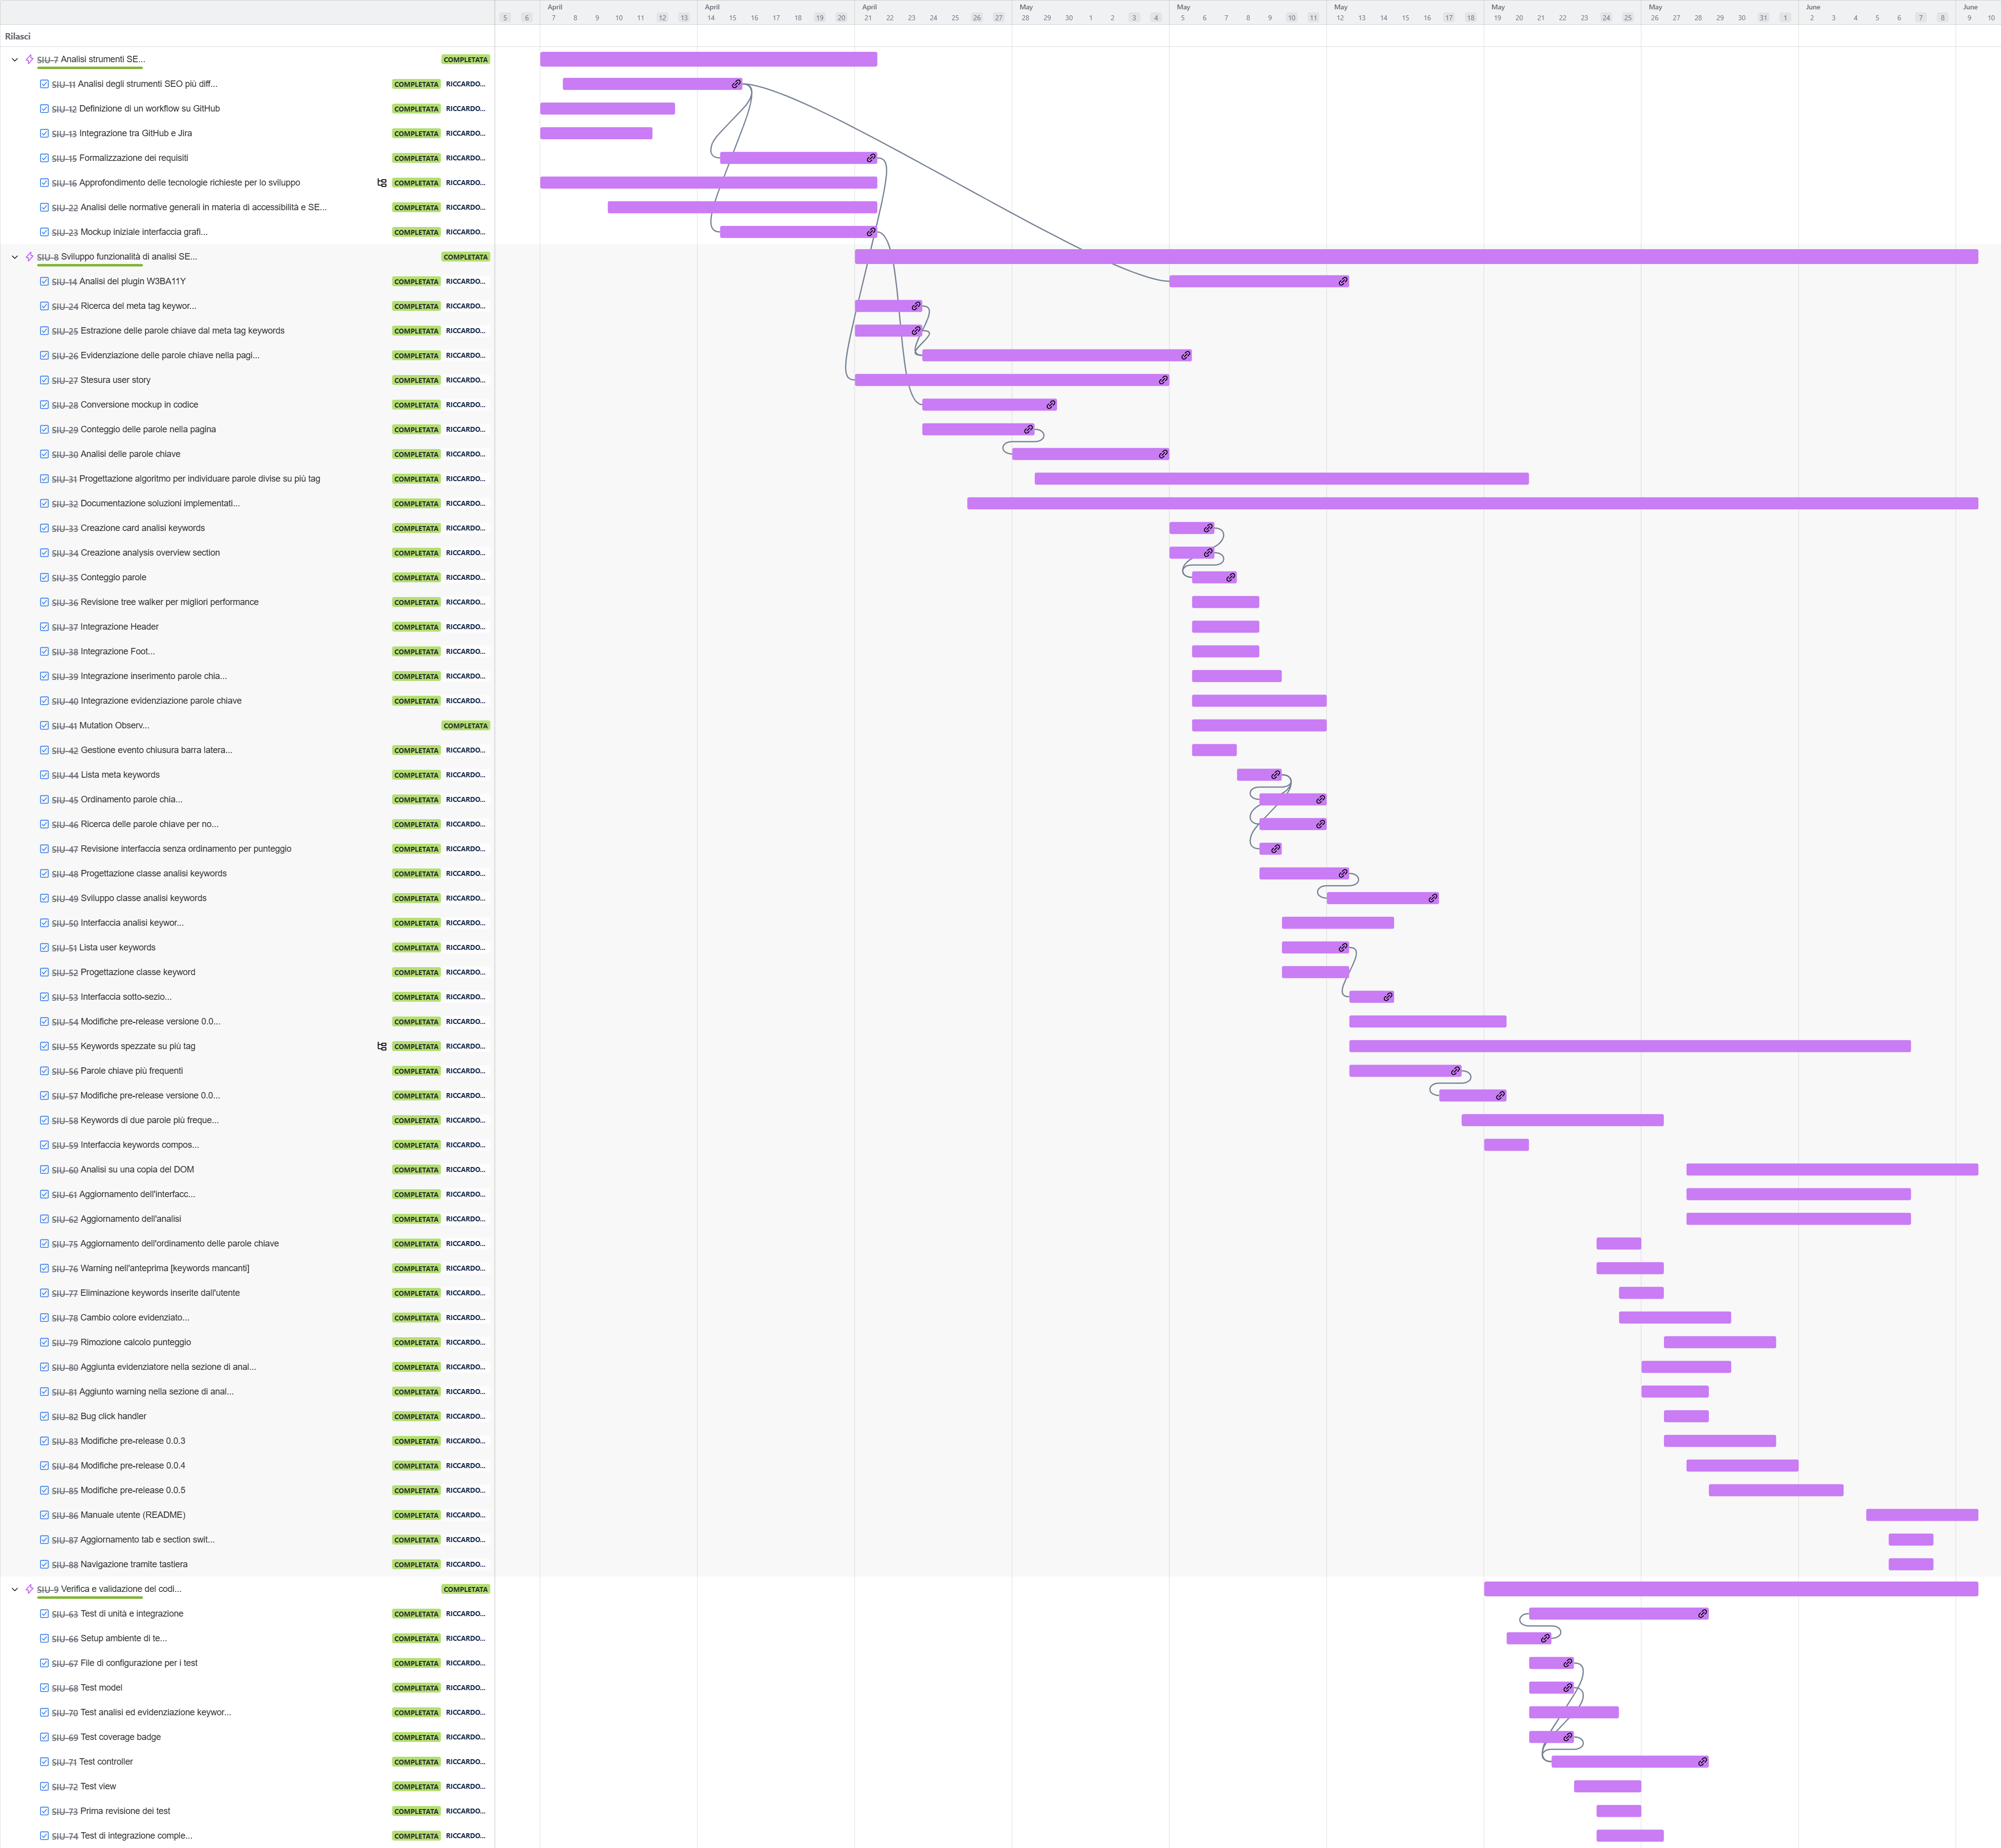
\includegraphics[width=0.8\columnwidth]{pianificazione/jira.png}} 
  \caption{Timeline Jira dal 07/04/2025 al 09/06/2025}
  \label{fig:timeline_jira}
\end{figure}

\section{Strumenti e tecnologie}
\label{sec:strumenti-tecnologie}

Di seguito sono elencati, in ordine alfabetico, i principali strumenti e tecnologie utilizzati durante lo svolgimento del progetto.

\subsection{Strumenti}

\subsection*{Chrome DevTools}

Gli strumenti per sviluppatori di Chrome consentono di ispezionare, \textit{debuggare} e modificare le pagine web. Sono integrati direttamente nel browser e fungono da console di \textit{debug}, offrendo agli sviluppatori la possibilità di individuare rapidamente eventuali errori. Il logo di Chrome DevTools è riportato in figura \ref{fig:logo_chrome_devtools}.

\begin{figure}[H]
  \centering 
  
\includegraphics[width=0.1\columnwidth]{strumenti-tecnologie/devtools_logo.png} 
  \caption{Logo di Chrome DevTools}
  \label{fig:logo_chrome_devtools}
\end{figure}

\subsection*{Codecov}

Codecov è un servizio di \textit{reporting} che monitora la copertura del codice, ovvero la percentuale di codice eseguito durante i test automatici. Nell’ambito del progetto di stage, è stato utilizzato per integrare queste informazioni direttamente nel flusso di lavoro su GitHub, in modo da garantire una copertura del codice uniforme per ogni \gls{pull request}. Inoltre, Codecov fornisce un \textit{badge} di stato utile ad arricchire la documentazione del \gls{repository}. Il logo di Codecov è riportato in figura \ref{fig:logo_codecov}.

\begin{figure}[H]
  \centering 
  
\includegraphics[width=0.1\columnwidth]{strumenti-tecnologie/codecov_logo.jpg} 
  \caption{Logo di Codecov}
  \label{fig:logo_codecov}
\end{figure}

\subsection*{Draw.io}

Draw.io è uno strumento \textit{web-based} utilizzato per la creazione di sketch e diagrammi. La piattaforma è \textit{open source} e mette a disposizione template personalizzabili. I progetti possono essere salvati localmente oppure online, grazie all’integrazione con Google Workspace (Google Drive) e Dropbox. In assenza di una connessione a Internet, è disponibile un'applicazione desktop per macOS, Windows e Linux. Nell’ambito del progetto di stage, Draw.io è stato impiegato per la realizzazione dei diagrammi dei \gls{use-case} e delle classi. Il logo di Draw.io è riportato in figura \ref{fig:logo_draw_io}.

\begin{figure}[H]
  \centering 
  
\includegraphics[width=0.1\columnwidth]{strumenti-tecnologie/draw_io_logo.jpg} 
  \caption{Logo di Draw.io}
  \label{fig:logo_draw_io}
\end{figure}

\subsection*{Figma}

Figma è uno strumento di progettazione e prototipazione, disponibile sia come servizio \textit{web-based} che come applicazione desktop. Due delle funzionalità più diffuse sono Figma Design, che consente di creare, condividere e testare i design in modo efficiente, e Dev Mode, che permette a designer e sviluppatori di collaborare strettamente per tradurre il design in codice. Nell’ambito dello stage, Figma è stato utilizzato per realizzare il \textit{mockup} dell’interfaccia grafica. Si è rivelato uno strumento di grande valore per la progettazione dell'interfaccia utente (UI) e dell’esperienza utente (UX), consentendo di analizzare lo spazio disponibile, organizzare gli elementi, scegliere i colori e costruire una base solida per lo sviluppo. Il logo di Figma è riportato in figura \ref{fig:logo_figma}.

\begin{figure}[H]
  \centering 
  
\includegraphics[width=0.1\columnwidth]{strumenti-tecnologie/figma_logo.png} 
  \caption{Logo di Figma}
  \label{fig:logo_figma}
\end{figure}

\subsection*{GitHub}

Github è un servizio \textit{web e cloud-based} per l'archiviazione, il versionamento e la condivisione del codice. Nell’ambito dello stage, è stato utilizzato per contribuire allo sviluppo di un progetto preesistente tramite la funzionalità di \textit{fork}, che consente di lavorare sul codice in modo isolato, per poi proporre le modifiche al \gls{repository} originale. GitHub permette anche di aprire spazi di discussione relativi al codice tramite \textit{issue} e \gls{pull request}, oltre a fornire strumenti per la gestione del progetto come \textit{board} e \textit{milestone}. Inoltre, consente di automatizzare i flussi di lavoro attraverso le \textit{GitHub Actions}. Il logo di GitHub è riportato in figura \ref{fig:logo_github}.

\begin{figure}[H]
  \centering 
  
\includegraphics[width=0.12\columnwidth]{strumenti-tecnologie/github_logo.png} 
  \caption{Logo di GitHub}
  \label{fig:logo_github}
\end{figure}

\subsection*{Google Docs}

Google Docs è un software \textit{web-based} per la scrittura e la condivisione di documenti. Nell’ambito del progetto di stage, è stato utilizzato per la redazione dei seguenti documenti: piano di lavoro, analisi degli strumenti \gls{seo}, analisi dei \gls{requisiti}, soluzioni progettuali e implementative. Il logo di Google Docs è riportato in figura \ref{fig:logo_google_docs}.

\begin{figure}[H]
  \centering 
  
\includegraphics[width=0.1\columnwidth]{strumenti-tecnologie/google_docs_logo.png} 
  \caption{Logo di Google Docs}
  \label{fig:logo_google_docs}
\end{figure}

\subsection*{Google Drive}

Google Drive è uno strumento \textit{web-based}, parte di Google Workspace, che consente di archiviare, organizzare, condividere e accedere in modo sicuro a file e cartelle ovunque, da qualsiasi dispositivo connesso a Internet. Nell’ambito del progetto di stage, Google Drive è stato adottato come “unica fonte di verità”, ovvero come raccolta centralizzata di tutto il materiale condiviso tra stagista e Proponente (piano di lavoro, appunti, link utili, analisi dei \gls{requisiti}, soluzioni progettuali, diagrammi e altro materiale correlato). Il logo di Google Drive è riportato in figura \ref{fig:logo_google_drive}.

\begin{figure}[H]
  \centering 
  
\includegraphics[width=0.1\columnwidth]{strumenti-tecnologie/google_drive_logo.png}  
  \caption{Logo di Google Drive}
  \label{fig:logo_google_drive}
\end{figure}

\subsection*{Google Forms}

Google Forms è uno strumento \textit{web-based} per la creazione di moduli, questionari, quiz e sondaggi. Nell’ambito del progetto di stage, è stato utilizzato per la creazione di un questionario \gls{sus} finalizzato alla valutazione dell’usabilità del software sviluppato. Il logo di Google Forms è riportato in figura \ref{fig:logo_google_forms}.

\begin{figure}[H]
  \centering 
  
\includegraphics[width=0.1\columnwidth]{strumenti-tecnologie/google_forms_logo.png} 
  \caption{Logo di Google Forms}
  \label{fig:logo_google_forms}
\end{figure}

\subsection*{Google Sheets}

Google Sheets è un software \textit{web-based} per la creazione e la condivisione di fogli di calcolo. Nell’ambito del progetto di stage, è stato utilizzato per memorizzare le risposte al questionario \gls{sus} e per creare una tabella di calcolo dei punteggi. Il logo di Google Sheets è riportato in figura \ref{fig:logo_google_sheets}.

\begin{figure}[H]
  \centering 
  
\includegraphics[width=0.1\columnwidth]{strumenti-tecnologie/google_sheets_logo.png} 
  \caption{Logo di Google Sheets}
  \label{fig:logo_google_sheets}
\end{figure}

\subsection*{Jira}

Jira è un'applicazione software sviluppata da Atlassian che consente agli utenti di gestire progetti, monitorare le attività e automatizzare i flussi di lavoro. È uno degli strumenti di gestione \textit{agile} più utilizzati, in particolare in contesti fortemente collaborativi, poiché risponde alle esigenze dei team di pianificare, monitorare, rilasciare e supportare software in modo sicuro. Nell’ambito dello stage, Jira è stato impiegato per la pianificazione e il monitoraggio delle tre fasi principali del progetto: analisi delle soluzioni esistenti, sviluppo e collaudo. L’integrazione con GitHub consente di tracciare i \textit{ticket} direttamente nell’ambiente di sviluppo e di automatizzarne la gestione. Inoltre, Jira mette a disposizione una \textit{timeline} che offre una panoramica immediata delle dipendenze tra le attività e del rispetto delle scadenze. Il logo di Jira è riportato in figura \ref{fig:logo_jira}.

\begin{figure}[H]
  \centering 
  
\includegraphics[width=0.18\columnwidth]{strumenti-tecnologie/jira_logo.png} 
  \caption{Logo di Jira}
  \label{fig:logo_jira}
\end{figure}

\subsection*{npm}

npm (Node Package Manager) è un gestore di pacchetti per JavaScript che consente di gestire le dipendenze di un progetto. Tutti i pacchetti sono definiti nel file di configurazione \textit{package.json}. Nell’ambito dello stage, npm è stato utilizzato per configurare i test automatizzati tramite Jest e per gestire il versionamento del progetto. Il logo di npm è riportato in figura \ref{fig:logo_npm}.

\begin{figure}[H]
  \centering 
  
\includegraphics[width=0.15\columnwidth]{strumenti-tecnologie/npm_logo.png}
  \caption{Logo di npm}
  \label{fig:logo_npm} 
\end{figure}

\subsection*{Visual Studio Code}

Visual Studio Code è un editor di codice sorgente, più leggero e flessibile rispetto a un ambiente di sviluppo integrato tradizionale. Combina la semplicità di un editor con \textit{feature} avanzate per sviluppatori, come il completamento del codice e altre funzionalità di assistenza alla scrittura. Il logo di Visual Studio Code è riportato in figura \ref{fig:logo_vscode}.

\begin{figure}[H]
  \centering 
  
\includegraphics[width=0.1\columnwidth]{strumenti-tecnologie/vscode_logo.png} 
  \caption{Logo di Visual Studio Code}
  \label{fig:logo_vscode} 
\end{figure}

\subsection{Tecnologie}

\subsection*{Chrome Extension APIs}

Le Chrome Extension APIs forniscono agli sviluppatori un insieme di interfacce che permettono di estendere e personalizzare le funzionalità del browser. Queste \gls{api} sono accessibili da qualsiasi componente dell’estensione. Consentono di accedere ai dati del browser, interagire con le schede, modificare il contenuto delle pagine web, memorizzare informazioni, gestire eventi e scambiare messaggi tra i componenti dell’estensione, ad esempio tra i \textit{background e i content script}. Il logo di Chrome Extension è riportato in figura \ref{fig:logo_chrome_extension}.

\begin{figure}[H]
  \centering 
  
\includegraphics[width=0.12\columnwidth]{strumenti-tecnologie/chrome_extension_logo.png} 
  \caption{Logo di Chrome Extension}
  \label{fig:logo_chrome_extension} 
\end{figure}

\subsection*{CSS}

CSS (Cascading Style Sheets) è un linguaggio utilizzato per definire lo stile e la formattazione di documenti scritti in linguaggi di markup come HTML o XML. Nell’ambito del progetto di stage, è stata adottata la versione CSS3. Il logo di CSS è riportato in figura \ref{fig:logo_css}.

\begin{figure}[H]
  \centering 
  
\includegraphics[width=0.25\columnwidth]{strumenti-tecnologie/css_logo.png} 
  \caption{Logo di CSS}
  \label{fig:logo_css} 
\end{figure}

\subsection*{HTML}

HTML (Hypertext Markup Language) è un linguaggio di markup utilizzato per definire la struttura e i contenuti delle pagine web. Nell’ambito del progetto di stage, è stata adottata la versione HTML5. Il logo di HTML è riportato in figura \ref{fig:logo_html}.

\begin{figure}[H]
  \centering 
  
\includegraphics[width=0.15\columnwidth]{strumenti-tecnologie/html_logo.png} 
  \caption{Logo di HTML}
  \label{fig:logo_html} 
\end{figure}

\subsection*{JavaScript}

JavaScript è un linguaggio di programmazione utilizzato per definire il comportamento e la logica delle pagine web. È un linguaggio multi-paradigma che può essere impiegato sia nella programmazione lato client che lato server (Node.js). JavaScript consente di aggiornare dinamicamente i contenuti HTML e gli stili CSS. Si integra perfettamente con \gls{framework} di test come Jest e strumenti di documentazione come JSDoc. È inoltre il linguaggio di riferimento per lo sviluppo di estensioni web. Il logo di JavaScript è riportato in figura \ref{fig:logo_javascript}.

\begin{figure}[H]
  \centering 
  \includegraphics[width=0.15\columnwidth]{strumenti-tecnologie/js_logo.png} 
  \caption{Logo di JavaScript}
  \label{fig:logo_javascript} 
\end{figure}

\subsection*{Jest}

Jest è un \gls{framework} di test per JavaScript, utilizzato per la progettazione, lo sviluppo e l’esecuzione di test di unità e di integrazione. Permette di definire suite di test efficienti e isolate, senza richiedere configurazioni complesse, anche quando viene integrato in progetti già avviati. Aggiungendo il flag \verb|--coverage|, è possibile generare un report sulla copertura del codice e inviare i risultati a strumenti di terze parti come Codecov. Nell’ambito del progetto di stage, Jest è stato utilizzato insieme alla libreria Jest DOM per ottenere una copertura completa del codice. Il logo di Jest è riportato in figura \ref{fig:logo_jest}.

\begin{figure}[H]
  \centering 
  
\includegraphics[width=0.1\columnwidth]{strumenti-tecnologie/jest_logo.png}
  \caption{Logo di Jest}
  \label{fig:logo_jest} 
\end{figure}

\subsection*{Librerie di icone}

Per l’interfaccia grafica sono state utilizzate icone provenienti da tre librerie, i cui loghi sono riportati in figura \ref{fig:loghi_librerie_icone}:
\begin{itemize}
  \item \textbf{Font Awesome}: una vasta libreria di icone vettoriali gratuite e a pagamento;
  \item \textbf{Heroicons}: una raccolta di icone \gls{svg} realizzate a mano dai creatori di \textit{Tailwind CSS};
  \item \textbf{Remix Icon}: una libreria \textit{open source} di icone vettoriali progettate per designer e sviluppatori.
\end{itemize}

\vspace{5pt}
\begin{figure}[H]
  \centering
  \begin{minipage}{0.3\columnwidth}
    \centering
    
\includegraphics[width=0.6\columnwidth]{strumenti-tecnologie/heroicons_logo.jpg} 
  \end{minipage}
  \hfill
  \begin{minipage}{0.3\columnwidth}
    \centering
    
\includegraphics[width=0.2\columnwidth]{strumenti-tecnologie/font_awesome_logo.jpg} 
  \end{minipage}
  \hfill
  \begin{minipage}{0.3\columnwidth}
    \centering
    
\includegraphics[width=0.6\columnwidth]{strumenti-tecnologie/remixicon_logo.jpg} 
  \end{minipage}
  \caption{Loghi delle librerie di icone: Heroicons, Font Awesome, Remix Icon}
  \label{fig:loghi_librerie_icone}
\end{figure}
\vspace{5pt}

\subsection*{Manifest (manifest.json)}

Il file \textit{manifest.json} svolge un ruolo cruciale nello sviluppo di estensioni web, poiché consente agli sviluppatori di definire le funzionalità dell’estensione e le autorizzazioni richieste. Si tratta di un file di configurazione in formato \gls{json} che specifica una serie di metadati, tra cui i permessi, le risorse necessarie, i \textit{background e i content script}.

\subsection*{Stopword (stopword.js)}

Stopword è un modulo JavaScript che consente di rimuovere le \gls{stopword} da un testo. Oltre alla funzione \textit{removeStopwords}, l’\gls{api} mette a disposizione identificatori univoci per accedere agli array di \gls{stopword} associati a lingue specifiche, con supporto verificato per oltre 60 lingue. Il modulo è distribuito con licenza \textit{MIT}.